% 202010??
\documentclass[env.tex]{subfiles}
\begin{document}

\begin{figure}[H]
    \centering
    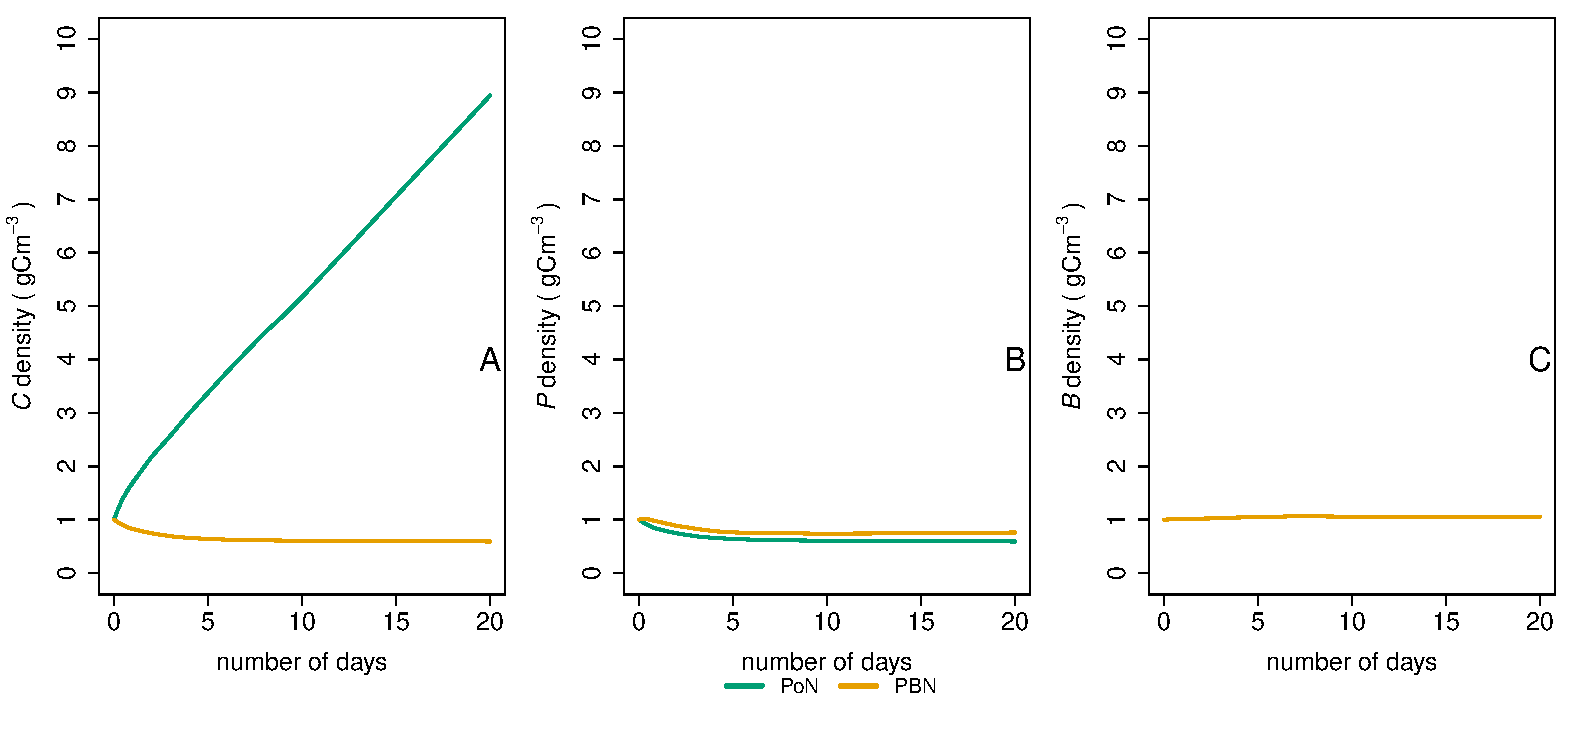
\includegraphics[width=\linewidth]{result/Sample.pdf}
    \caption[Median carbon content in destructive systems]{Median carbon content in destructive systems.  \textbf{(A)}, \textbf{(B)} and \textbf{(C)} show carbon densities in respective carbon pools since establishment.  Initial carbon densities for \PoN\ were [1,1,0]\den\ ($C$, $P$, $B$) and that for \PBN\ were [1,1,1]\den\ modeled from Eq.\ref{eq:PBH}.  Note that \PoN\ carbon accumulation was linear after establishment.}
    \label{f:destCarbon}
\end{figure}

\begin{figure}[H]
    \centering
    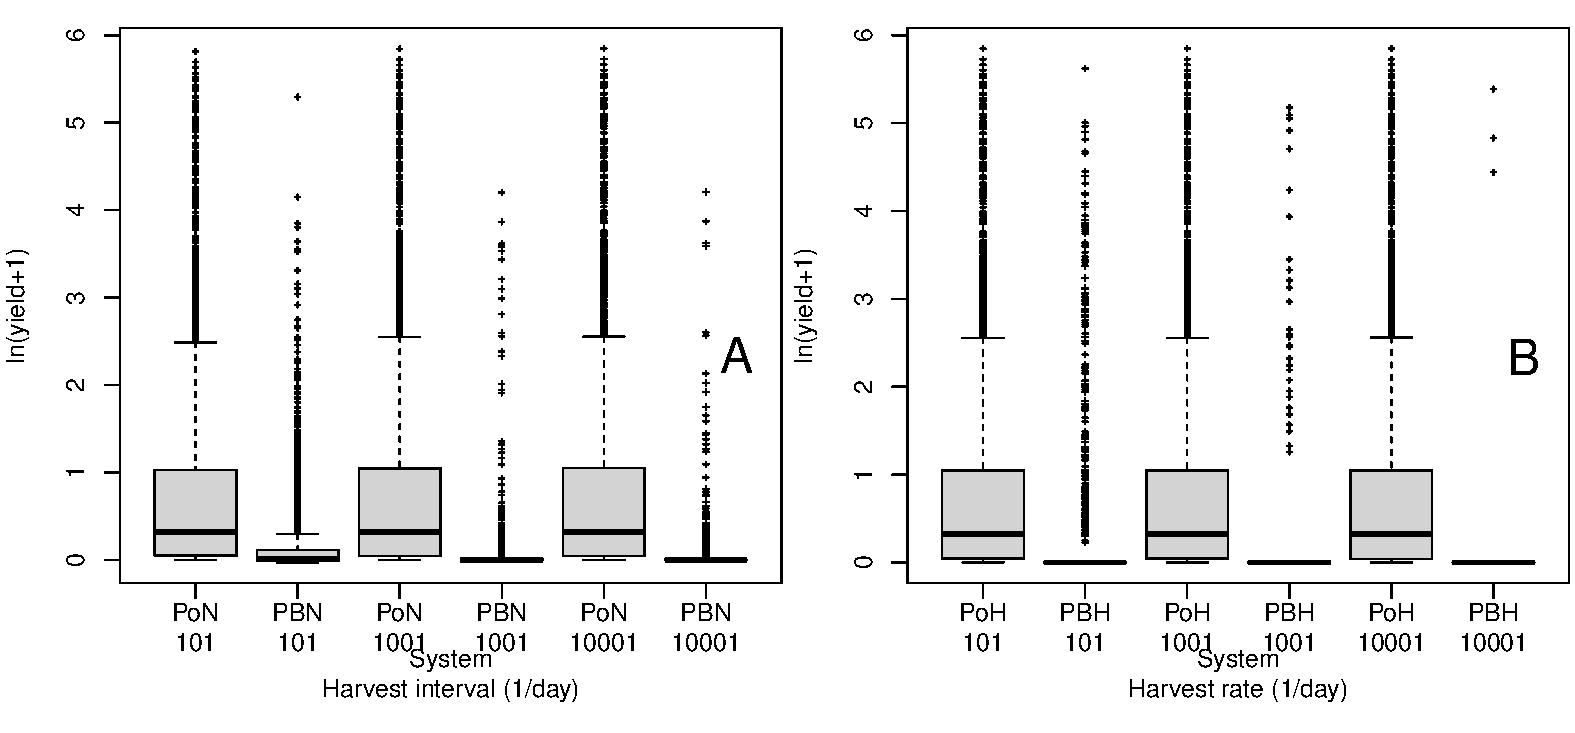
\includegraphics[width=\linewidth]{result/Harvest.pdf}
    \caption[Yield flux distribution by harvest mode]{Log distribution of feasible scenarios at selected harvest interval/rates.  Unfeasible scenarios have caused some boxes represent a smaller sample size than the initial 5500.  Most boxes had a sample size of 5500, except \PBN\ day 50 (n=5454) and \PBH\ systems in \textbf{(B)} ($x$=100 \dayU, n=184; $x$=1000 \dayU, n=31; $x$=10K \dayU, n=3).  Note that \PoN\ day 0.5 in \textbf{(A)} was the only box with median significantly different (pairwise Wilcox p$\ll$0.01) from other \phy-only distributions.\pAExplain\  Raw yields are incremented by 1 because the minimum yield is larger than -1 and there are 0 yield in some scenarios.  Hence log of incremented yields shifts and bounds the distribution between -1 and 6.}
    \label{f:ydByHarv}
\end{figure}

\begin{figure}[H]
    \centering
    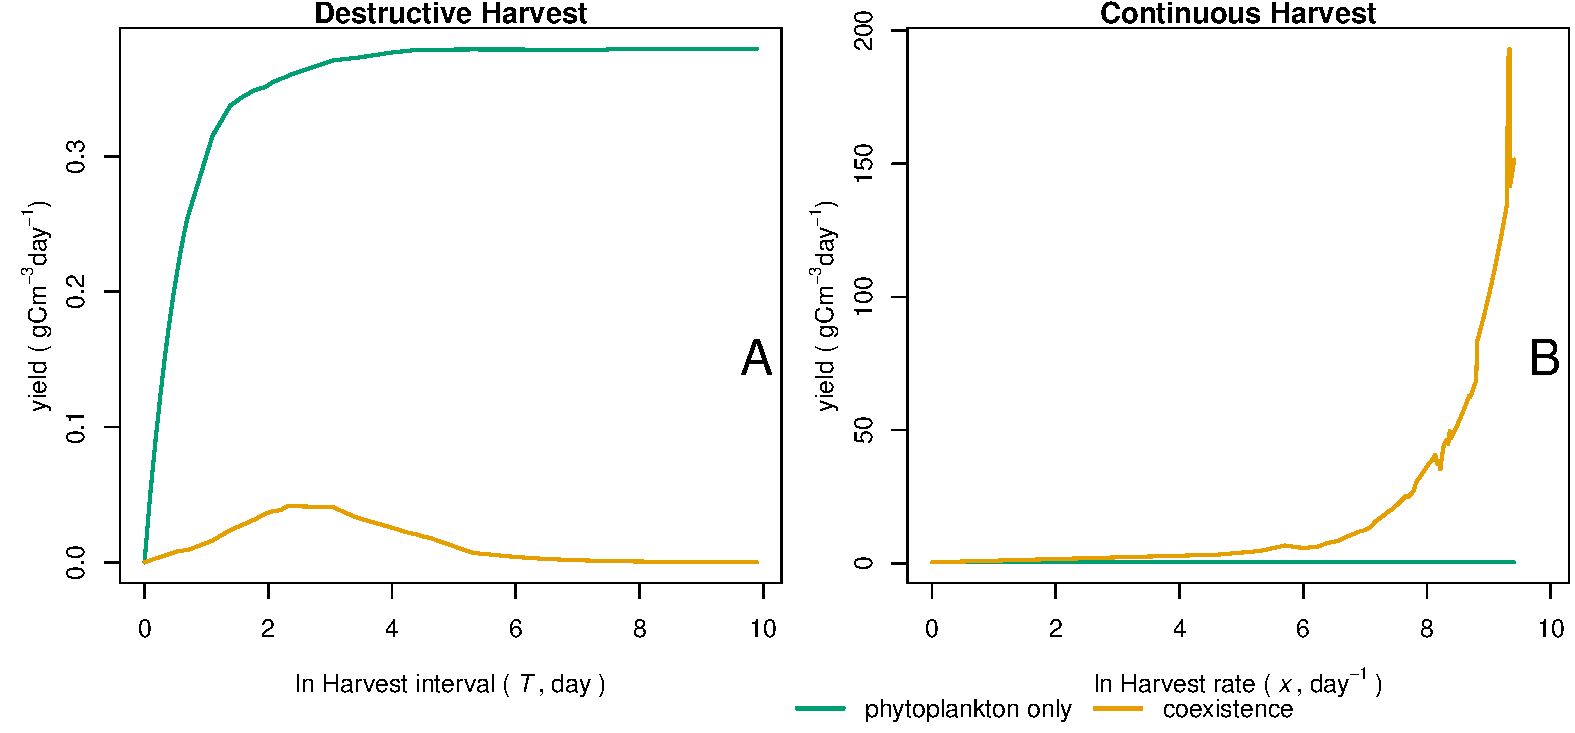
\includegraphics[width=\linewidth]{result/DailyYield.pdf}
    \caption[Median daily carbon yield across systems]{Median daily carbon yield across systems.  Panel \textbf{(A)} shows yield as a function of harvest interval for destructive harvest scenarios.  Panel \textbf{(B)} shows log yield as a function of harvest rate for continuous harvest scenarios.  Unfeasible data was treated as invalid data.  Note that the \phy-only system numerical value is the same between \textbf{(A)} \& \textbf{(B)} but cannot be seen due to the scales.  Also note that feasible scenarios have the highest median yield compared to all systems \textbf{(B)}.\lnExplain}
    \label{f:ydDaily}
\end{figure}

\begin{figure}[H]
    \centering
    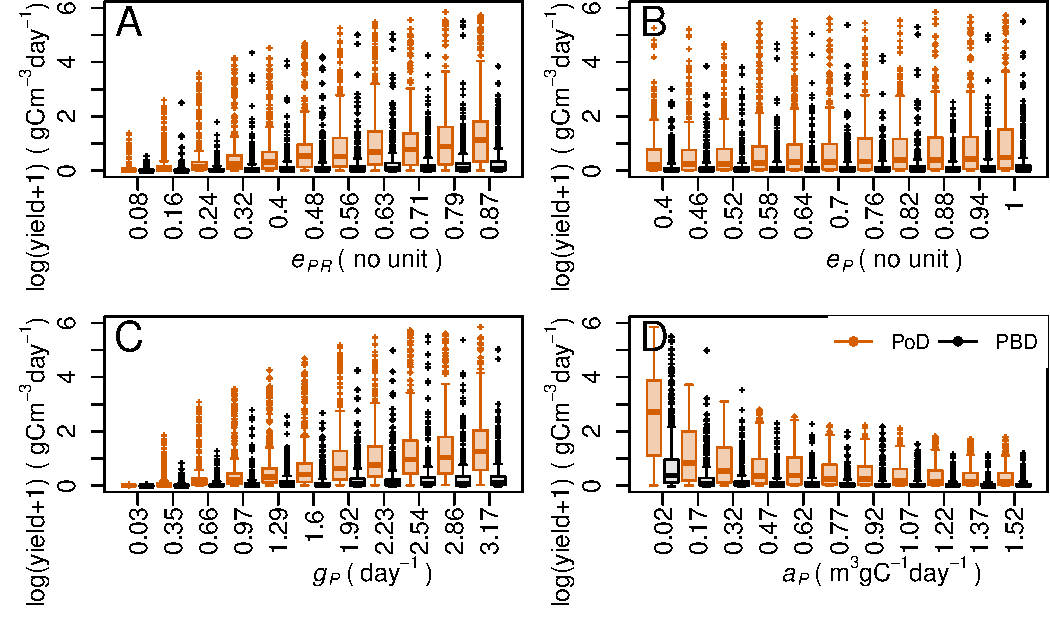
\includegraphics[width=\linewidth]{result/bacEff1.pdf}
    \caption[Log yield flux comparisons between feasible \phy-only and \pbs s]{Log yield flux comparisons between \phy-only and \pbs s on \phy\ parameters.  All parameters had significant influence on both \PoN\ and \PBN\ (Wilcox p$\ll$0.01 between extreme parameter values on both systems).  Carbon yield in $\ePR$ and $\gP$ peaked at a high value (\textbf{A}\&\textbf{C}).\lnExplain}
    \label{f:bacEffect}
\end{figure}

\begin{figure}[H]
    \centering
    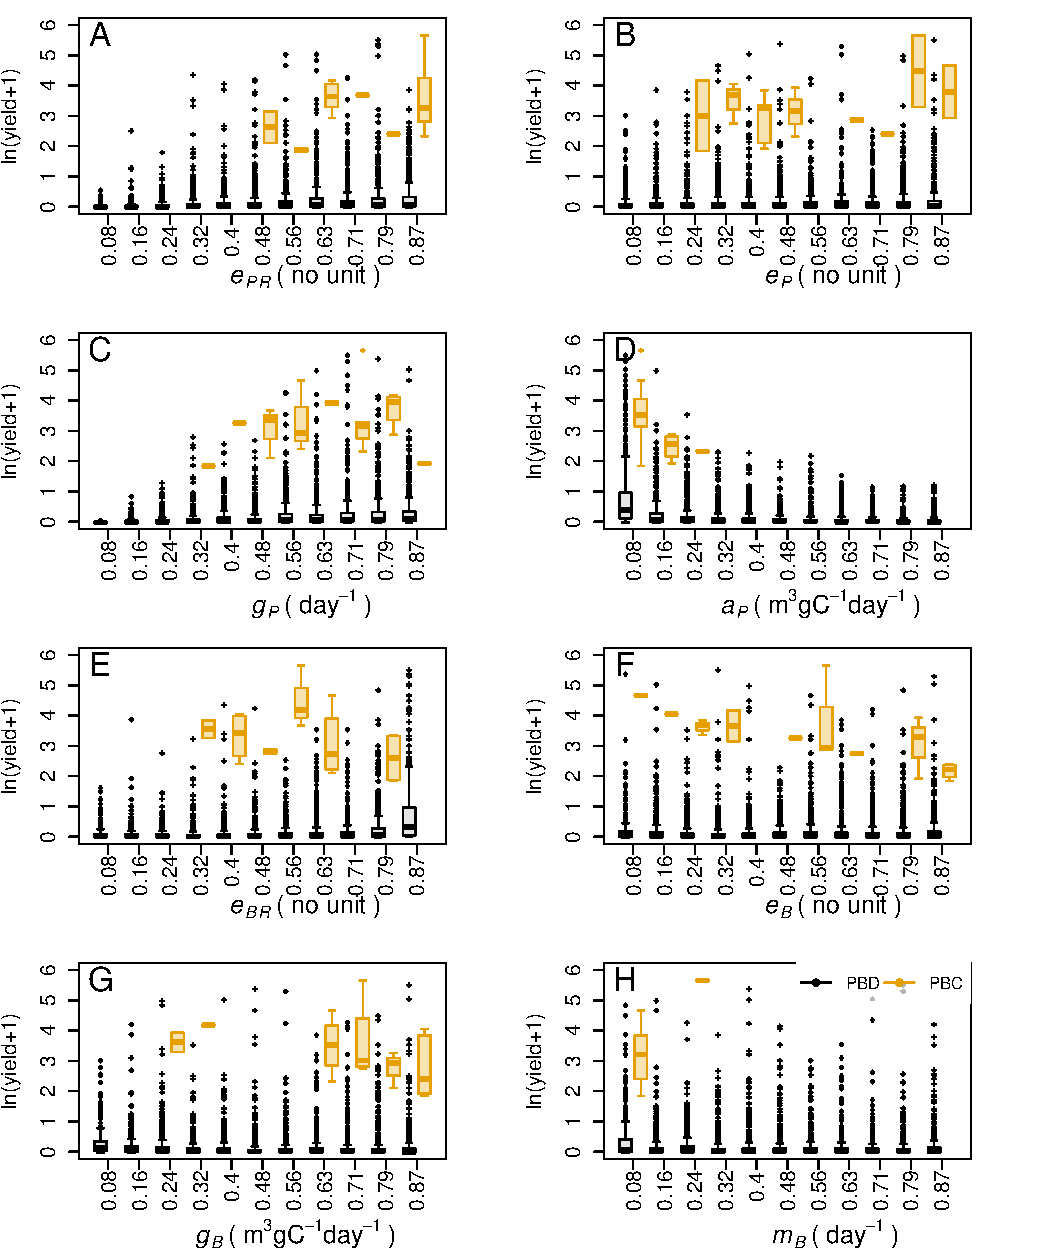
\includegraphics[width=\linewidth]{result/harvB.pdf}
    \caption[Log yield flux comparisons between feasible \pbs s]{Log yield flux comparisons between feasible \pbs s.  \PBH\ feasible distributions were not continuous across parameter ranges with small number of scenarios (n=19) but yielded higher than that of \PBN.  All parameters had significant influence on both \PBN\ and \PBH\ (Wilcox p$\ll$0.01 between extreme parameter values on both systems).\lnExplain}
    \label{f:harvPB}
\end{figure}

\end{document}